\documentclass[conference]{IEEEtran}
\usepackage{cite}
\usepackage{amsmath,amssymb,amsfonts}
\usepackage{algorithmic}
\usepackage{graphicx}
\usepackage{textcomp}
\usepackage{xcolor}
\usepackage{multirow}
\usepackage{booktabs}
\def\BibTeX{{\rm B\kern-.05em{\sc i\kern-.025em b}\kern-.08em
    T\kern-.1667em\lower.7ex\hbox{E}\kern-.125emX}}
\begin{document}

\title{A review on Generative Learning in Computer Vision}

\author{\IEEEauthorblockN{Pathan Faisal Khan}
\IEEEauthorblockA{Letterkenny Institute of Technology \\
Port Road, Letterkenny\\
Co. Donegal, Ireland \\
L00151142@student.lyit.ie}}

\maketitle

\begin{abstract}

\end{abstract}

\begin{IEEEkeywords}
component, formatting, style, styling, insert
\end{IEEEkeywords}

\section{Introduction}
Artificial intelligence has made it possible for computers to learn from experiences and perform simple tasks which a human can easily do. Visual perception by human-like object recognizing abilities is once such task which scientists have been able to teach computers. In the past few years due to advancement and innovation in computing power especially unlocking GPU based distributed computing, computer scientists have achieved good success in able to teach computers to do complex tasks beyond classification like object detection, image segmentation, object tracking, and event detection. Computer Vision (CV) has since been used in numerous ways ranging from automated cars to quality check at factories which usually required an expert to manually check the production line.

With such advancements, the need for data is never ending. CV models running on neural networks require huge amount labeled training data to train them. But the problem lies in finding suitable high-quality data. Manual scavenging and labelling of data is not an ideal approach as it is costly to do so. The only option left for computer scientists is to produce high quality artificial data either from scratch or by manipulating existing data. Generative learning is one such popular way to generate artificial data. This paper will look at different generative methods introduced lately.

The rest of the paper is organized as follows-- Section \ref{lr} will provide an overview of generative learning. Section \ref{techniques} will cover recent techniques used for generative learning. Section \ref{comparison} will provide a comparison of different techniques discussed in section \ref{techniques}. Finally, section \ref{conclusion} will provide some remarks to conclude the paper. 

\section{Generative Learning}
\label{lr}
\subsection{Background}
Computer scientists has contributed a lot of research towards generating synthetic visual data. With such techniques, computer scientists has been able to generate data which is almost indistinguishable by a human eye. This fast availibility of generated data has made it possible to solve a lot of modern problems in deep learning.

There has been some generative techniques around in this field of deep learning. In 2014, Goodfellow et al. published a paper on Generative Adversarial Networks (GANs) \cite{b1}. This state-of-the-art technique proved to be a major break-through in deep learning especially in CV. GANs has since then been applied in numerous fields including Natural Language Processing (NLP) and computer vision. This family of deep learning methods has become quite popular due to its good results. This review paper provides a survey on recent adaptations of GAN alongwith the first-original version often called as vanilla GAN. Autoencoders is a class of unsupervised neural networks which is also a popular method to generate data with some applications dating back to the 80s \cite{b2, b3}. Variational Autoencoders (VAEs) in specific is a generative technique.

\subsection{Taxonomy}
The following Table \ref{tab:taxonomy_table} presents taxonomy of different generative learning techniques--

\begin{table*}[]
    \caption{Taxonomy and citations of Generative Learning techniques}
    \label{tab:taxonomy_table}
    \centering
    \begin{tabular}{l l l}
        \toprule
        \multicolumn{2}{l}{Technique} & Citations \\ 
        \midrule
  
        \multirow{2}{*}{} & Conditional GAN & \begin{tabular}[c]{@{}l@{}} \cite{b4}\\
        \end{tabular}\\ 
 
        \cline{2-3} 
        \multirow{2}{*}{} & Progressive GAN & \begin{tabular}[c]{@{}l@{}} \cite{b12}\\
        \end{tabular}\\ 
 
        \cline{2-3} 
        \multirow{2}{*}{} & Deep Convolutional GANs (DCGAN) & \begin{tabular}[c]{@{}l@{}} \cite{b5}\\
        \end{tabular}\\  
    
        \cline{2-3} 
        \multirow{2}{*}{} & Auxiliary Classifier GAN & \begin{tabular}[c]{@{}l@{}} \cite{b7}\\
        \end{tabular}\\ 
        
        \cline{2-3} 
        Generative Adversarial Networks &  Info GANs  & \begin{tabular}[c]{@{}l@{}} \cite{b6}\\
        \end{tabular}\\ 
        
        \cline{2-3} 
        \multirow{2}{*}{} & 3D-GAN & \begin{tabular}[c]{@{}l@{}} \cite{b8}\\
        \end{tabular}\\  
 
        \cline{2-3} 
        \multirow{2}{*}{} & PacGAN & \begin{tabular}[c]{@{}l@{}} \cite{b9}\\
        \end{tabular}\\ 
 
        \cline{2-3} 
        \multirow{2}{*}{} & Pix2PixGAN & \begin{tabular}[c]{@{}l@{}} \cite{b10}\\
        \end{tabular}\\

        \cline{2-3} 
        \multirow{2}{*}{} & Cycle-GAN & \begin{tabular}[c]{@{}l@{}} \cite{b11}\\
        \end{tabular}\\ 

        \cline{2-3} 
        \multirow{2}{*}{} & Text-to-Image Synthesis (StackGAN) & \begin{tabular}[c]{@{}l@{}} \cite{b13}\\
        \end{tabular}\\ 

        \cline{2-3} 
        \multirow{2}{*}{} & Super-Resolution GAN & \begin{tabular}[c]{@{}l@{}} \cite{b14}\\
        \end{tabular}\\ 

        \midrule

        Autoencoders & Variational Autoencoders (VAEs) & \cite{b15}   \\ 
        
        \bottomrule
    \end{tabular}
\end{table*}

\section{Techniques}
\label{techniques}

\subsection{Generative Adversarial Networks (GANs)}
Goodfellow et al. developed this state-of-the-art class of neural networks with two key components; a generator and a discriminator. The generator is a neural network which takes a random vector input usually a noise and generates a new plausible output out of it in the domain. This vector input is taken from a Gaussian distribution. A Gaussian or normal distribution is a probability distribution around a mean, which signifies the data around the mean is more frequent as compared to data points away from the mean. A Gaussian distribution shows a bell curve when plotted. The vector is referred as a latent space which means significant variables but not explicity visible. Due to the fact that it uses random vector sample every time, the model becomes stochastic, the output will be non-deterministic every time. The generator makes unlimited samples out of it. The discriminator, a classification model, then takes input from the training dataset as well as output from the generator model and attempts to identify source of the input, whether it is from the training dataset or from the generator generated ouput. Both models are meant to compete with each other, the generator has to fool the discriminator into incorrectly classifying its sample as a real sample from the training set and the discriminator has to make itself perfect in correctly classifying input samples. The generator and the discriminator are both trained alongwith. When the discriminator predicts the class of the input sample, it is tweaked to perform better for the next sample, likewise the generator is updated to create samples which will fool the discriminator. Even though GAN is an unsupervised learning technique but this architecture of it is designed as a supervised learning technique. The generator model is then used discarding the discriminator model. The following figure \ref{fig1} describes the working of a GAN.

\begin{figure}[!h]
    \centerline{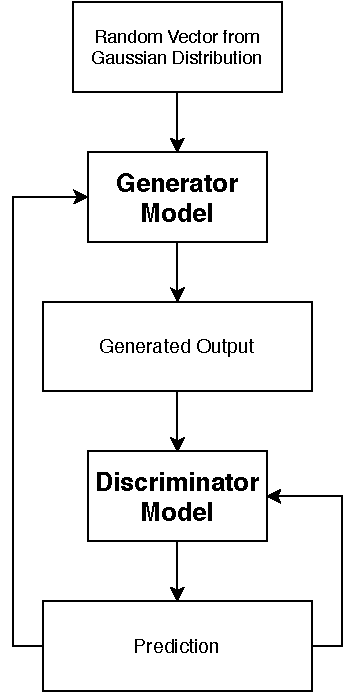
\includegraphics[scale=0.6]{figures/GAN.pdf}}
    \caption{End-to-end process of the Vanilla GAN}
    \label{fig1}
\end{figure}

\subsubsection{Conditional GAN}
Conditional GAN is an extension of GAN proposed by Mirza et al. in 2014 \cite{b4}. It works on the principal of conditional probability which is defined as the probability of an event given another event mathematically represented as $P(A|B)$ which translates to probability of $A$ given $B$. Conditional GAN is conditioned using extra information which is passed to the generator as well as to the discriminator. This extra information can be any supplementary information like image labels. The discriminator gets the extra information alongwith the input from generator. One of the applications of conditional GAN is generating image of a person given its gender. The following figure \ref{fig2} describes the working of a conditional GAN.

\begin{figure}[!h]
    \centerline{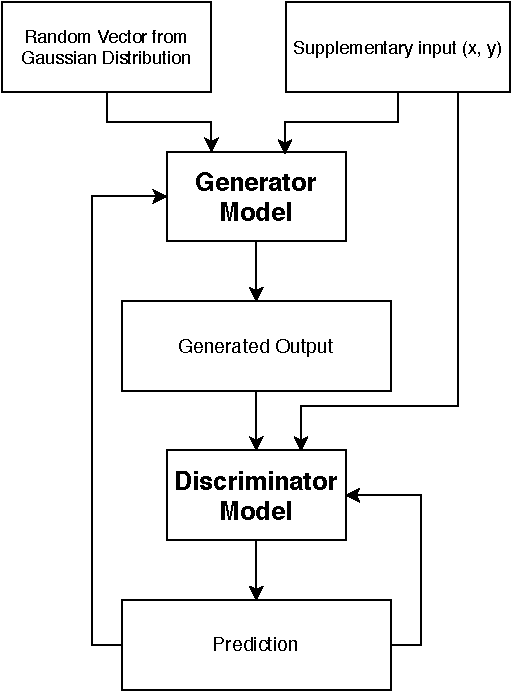
\includegraphics[scale=0.6]{figures/CGAN.pdf}}
    \caption{End-to-end process of the conditional GAN}
    \label{fig2}
\end{figure}

\subsubsection{Progressive GAN}
Karras et al in 2017 published a paper introducing progressive GAN \cite{b12}. According to the authors of the paper, they proposed a novel training technique where the generator and discriminator grow progressively as they train themselves. Growing progressively means adding more layers to themselves to fine tune the model. With this approach, the training time decreases. The generator produces low quality images and as more layers are added it fine tunes the model resulting in high quality images. This progressive learning technique allows the model to gradually discover large scale composition of the image and then focus on improving the fine details of the image. New layers are added in such a way that it does not drastically affect the fine tuned network. Figure \ref{fig3} shows how layers are added to both the generator and discriminator together.

\begin{figure}[!h]
    \centerline{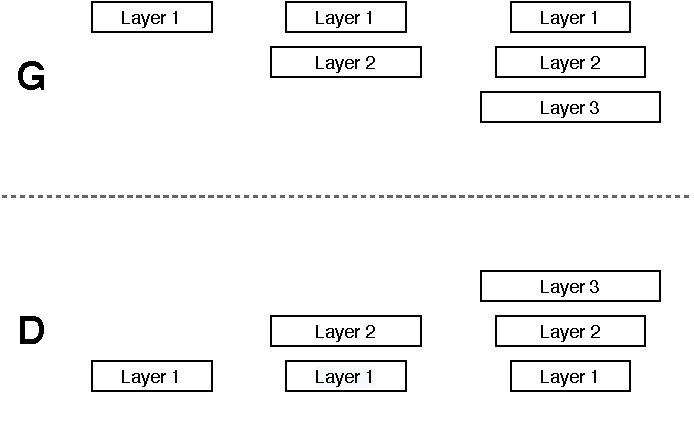
\includegraphics[scale=0.7]{figures/PGAN.pdf}}
    \caption{Addition of layers in every iteration of progressive GAN}
    \label{fig3}
\end{figure}

\subsubsection{Deep Convolutional GAN (DCGAN)}

\subsubsection{Auxiliary Classifier GAN}

\subsubsection{3D-GAN}

\subsubsection{Info GAN}

\subsubsection{PacGAN}

\subsubsection{Pix2PixGAN}

\subsubsection{Cycle-GAN}

\subsubsection{Text-to-Image Synthesis (StackGAN)}

\subsubsection{Super-Resolution GAN}

\subsection{Autoencoders}

\subsubsection{Variational Autoencoders (VAEs)}

\section{Comparison}
\label{comparison}

\section{Conclusion}
\label{conclusion}

\begin{thebibliography}{00}
\bibitem{b1} Goodfellow, I.J., Pouget-Abadie, J., Mirza, M., Xu, B., Warde-Farley, D., Ozair, S., Courville, A., Bengio, Y., 2014. Generative Adversarial Networks. arXiv:1406.2661 [cs, stat].

\bibitem{b2} Ballard, D.H., 1987. Modular learning in neural networks, in: Proceedings of the Sixth National Conference on Artificial Intelligence - Volume 1, AAAI’87. AAAI Press, Seattle, Washington, pp. 279–284.

\bibitem{b3} Rumelhart, D.E., Hinton, G.E., Williams, R.J., 1986. Learning internal representations by error propagation, in: Parallel Distributed Processing: Explorations in the Microstructure of Cognition, Vol. 1: Foundations. MIT Press, Cambridge, MA, USA, pp. 318–362.

\bibitem{b4} Mirza, M., Osindero, S., 2014. Conditional Generative Adversarial Nets. arXiv:1411.1784 [cs, stat].

\bibitem{b5} Radford, A., Metz, L., Chintala, S., 2016. Unsupervised Representation Learning with Deep Convolutional Generative Adversarial Networks. arXiv:1511.06434 [cs].

\bibitem{b6} Chen, X., Duan, Y., Houthooft, R., Schulman, J., Sutskever, I., Abbeel, P., 2016. InfoGAN: Interpretable Representation Learning by Information Maximizing Generative Adversarial Nets. arXiv:1606.03657 [cs, stat].

\bibitem{b7} Odena, A., Olah, C., Shlens, J., 2017. Conditional Image Synthesis With Auxiliary Classifier GANs. arXiv:1610.09585 [cs, stat].

\bibitem{b8} Wu, J., Zhang, C., Xue, T., Freeman, W.T., Tenenbaum, J.B., 2016. Learning a Probabilistic Latent Space of Object Shapes via 3D Generative-Adversarial Modeling.

\bibitem{b9} Lin, Z., Khetan, A., Fanti, G., Oh, S., 2018. PacGAN: The power of two samples in generative adversarial networks, in: Bengio, S., Wallach, H., Larochelle, H., Grauman, K., Cesa-Bianchi, N., Garnett, R. (Eds.), Advances in Neural Information Processing Systems 31. Curran Associates, Inc., pp. 1498–1507.

\bibitem{b10} Isola, P., Zhu, J.-Y., Zhou, T., Efros, A.A., 2018. Image-to-Image Translation with Conditional Adversarial Networks. arXiv:1611.07004 [cs].

\bibitem{b11} Zhu, J.-Y., Park, T., Isola, P., Efros, A.A., 2018. Unpaired Image-to-Image Translation using Cycle-Consistent Adversarial Networks. arXiv:1703.10593 [cs].

\bibitem{b12} Karras, T., Aila, T., Laine, S., Lehtinen, J., 2018. Progressive Growing of GANs for Improved Quality, Stability, and Variation. arXiv:1710.10196 [cs, stat].

\bibitem{b13} Zhang, H., Xu, T., Li, H., Zhang, S., Wang, X., Huang, X., Metaxas, D., 2017. StackGAN: Text to Photo-realistic Image Synthesis with Stacked Generative Adversarial Networks. arXiv:1612.03242 [cs, stat].

\bibitem{b14} Ledig, C., Theis, L., Huszar, F., Caballero, J., Cunningham, A., Acosta, A., Aitken, A., Tejani, A., Totz, J., Wang, Z., Shi, W., 2017. Photo-Realistic Single Image Super-Resolution Using a Generative Adversarial Network. arXiv:1609.04802 [cs, stat].

\bibitem{b15} Doersch, C., 2016. Tutorial on Variational Autoencoders. arXiv:1606.05908 [cs, stat].

\end{thebibliography}
\end{document}
